\documentclass{exam}
\usepackage[utf8]{inputenc}
\usepackage{fancyhdr}
\usepackage[]{tipa}
\usepackage{afterpage}
\documentclass{article}
\usepackage{amssymb}
\usepackage{amsmath}
%\usepackage{amsfonts}
%\usepackage{latexsym}
%\usepackage{mathrsfs}
\usepackage{color}
\def\0{{\bf 0}}
\def\I{\mathbb{ I}}
\newcommand{\squeezeup}{\vspace{-2mm}}
\newcommand{\morespace}{\vspace{+2mm}}

\title{LING 425: HISTORICAL LINGUISTICS}

\squeezeup \squeezeup
\date{Fall Semester 2016}
\author{Prof. Charles Boberg}
\usepackage{natbib}
\usepackage{graphicx}

\begin{document}



\pagestyle{fancy}
\fancyhf{}
\rhead{Notes: LING 425 Historical Linguistics}
\lhead{Sophia Davis}
\pagenumbering{arabic}

\maketitle



\section*{Tuesday, 6 September 2016: Introduction}

\noindent \textbf{Historical linguistics} is defined as ``the study of the history and development of languages". It is interdisciplinary, and often draws from the fields of archaeology and anthropology. Change is inherent to language; thus, any theory of language that does not account for change in incomplete. The goal of historical linguistics is to identify and explain the principles that govern language change, and use those principles to constrain theories about language change. Applications: identifying related language families and proposing hypothetical proto languages; determining which language changes are likely to occur in the future; identifying the social mechanisms that drive language change.
\fancyfoot[C]{\thepage}


\paragraph{Related Terms} Linguistic fields can be separated into one of two subcategories, \textbf{diachronic} and \textbf{synchronic}. The latter examines a language at a given point in time, whereas the former examines the differences in a language in different times. \textbf{Philology} (Greek, ``love of words"), is defined as ``the branch of knowledge that deals with the structure, historical development, and relationships of a language or languages". \textbf{Etymology} is the study of word origins. \par
 


\paragraph{Common Problems} It is often difficult to examine language change due to the paucity of written record for most languages. Also, written records fail to illustrate many aspects of a language, such as pronunciation. (The extent of our understanding largely hinges on whether the writing system is phonetic or not; for instance, Chinese is not phonetic and English and French are only partially). Nearly all writing systems are phonemic, and only indicate contrasts. However, written texts are valuable for observing certain other aspects of language, such as syntax and lexicon. \par Additionally, pervasive literacy is a modern phenomenon. Old texts almost certainly do not reflect the full range of language, but only the type of language used by an educated upper class in certain formal situations. 


\paragraph{Attitudes} Language change, although inevitable, is often met with resistance. Older language forms are often regarded as the ``better" or ``pure" forms, whereas newer language is considered degenerate and corrupt. This is true regardless of time period or geographical location. Relatively few celebrate language change, with the exception of slang that is seen to define the cultural ethos of a group or generation. \par Even now, language is morphing. Consider the drop in the use of ``whom". Or the substitution of ``was like" for ``said". Many changes are ephemeral, but many others stick and are passed down to future generations. Many people consider their language as stable, when this is never the case. 



\section*{Thursday, 7 September 2016: Introduction (con't)}

Many linguistic changes are documented in the \textit{Journal of Modern Linguistics}. Examples from recent issues include ``Netflix and chill", ``sharewashing", and ``Thanks, Obama". (Most of these words will most likely not last very long.) These changes in lexicon force lexicologists to habitually add and trim words from dictionaries. 

\begin{center} 
\paragraph{Evolution of English }
\end{center}


\noindent \textbf{\\Old English} Exemplified by \textit{Beowulf}, circa 750 A.D. 
\begin{itemize}

\item Totally incomprehensible to speakers of 21c English. Certain words (life, world) are relatively unchanged, however. Uses alliteration rather than modern rhyme scheme. 
\item Contained rich declensions (variation in noun forms), similar to German. For instance, it distinguished between 3 genders (neutral, female, male) and many cases (nomative, accusative, generative, dative), and plurality, whereas modern English only distinguishes between singular and plural forms. Also had more conjugations, whereas modern English only preserves one unique form (-s on the present plural singular). Some archaic forms from OE preserved in ME: consider difference in ``ride" ``he rode" vs. ``he has ridden". This distinction is not present in new verbs e.g. there is no difference between ``she googled" and ``she had googled". 

\end{itemize}

\noindent \textbf{\\Middle English} Exemplified by \textit{Canterbury Tales}, 1387 A.D. 
\begin{itemize}

\item Disappearance of Anglo-Saxon graphemes. Familiar rhyming scheme (couplets). Much more recognizable. 
\item Change in language due to Norman conquest (example of an extralinguistic event with linguistic consequences): vikings, many who had spent time in France and absorbed French language/culture; as a result, many French vocabulary words were borrowed into English. This was a lasting change; an estimated one third to one half of modern English vocabulary is derived from French. 
\item Not shown in text: pre-Great Vowel Shift, so although spelling is same as modern English, pronunciation was quite different. 
\item Many nouns feature a word final vowel, and declensions (though even these are relatively simplified when compared to Old English). 
\item Middle English was unstandardized, and had many alternate spellings. 
\end{itemize}

\noindent \textbf{\\Early Modern English} exemplified by \textit{King James Bible}, 1611 A.D. 
\begin{itemize}
\item Totally understandable by speakers of modern English. Still commonly in use today. 
\item Considered a ``high point" of English prose. 
\item Also reflective of a non linguistic event (Protestant reformation). Emphasis on having a direct path with god, which led to translation of bible into local languages to be accessible to the plebians. 
\item Given the formal nature of the subject matter, it is most likely exemplifies language that is old fashioned for its time. (For instance the ye/your vs thee/thou distinction is sometimes ignored in Shakespeare's works, indicating that its use is already somewhat dated.)
\item Post great vowel shift; disappearance of superfluous e's
\end{itemize}

 
\section* {Tuesday, 13 September 2016: Borrowing}


\noindent World War Two: Many Canadian/American soldiers who went to Britain; exposure to various dialects. After, US rose to `superpower' status, and US troops were stationed everywhere, spreading American English wordwide. This helped push English to the status of global dominance. 

Changes in language include changes in sound, grammar, morphology, lexicon. Sound change is the best studied aspect of sound change. Often a change in contrast, or phonological change, or phonetic change. The \textbf{Neo-grammarian hypothesis} postulated that sound change is systematic, and it operates without exceptions. 

If change is random, then we cannot assume that the systematic correspondences that we identify between languages. The assumption of regularity allows loanwords to be identified as exceptions to sound change. There are two methods of identifying loanwords in a language. First, linguists can identify source of loanword in another language; secondly, it should also be obvious that the word did not undergo the changes in the host language before it was borrowed. Or, it is possible that the law did not apply in that case, and the Neo-Grammarian hypothesis of regular sound change is wrong. 

Hypothesis of sound change are testable: theories about sounds that should have changed over times can be tested with new data from various time periods in the language. 

In old changes, it's hard to know whether apparent regularity operated throughout he process of the change or was a result of a gradual diffusion of a change through the available vocabulary. For instance, if p became b, we don't know if it happened one word at a time or all at once; we do not know the mechanism by which regularity resulted. 

Sound changes are notated using a series of abridged notations, eliminating the need for verbose descriptions. 


$$X >Y$$
\begin{center}
X becomes Y.
\end{center}


Textbook distinguishes \textbf{conditioned} and \textbf{unconditioned} changes. The above is unconditional. Conditional changes are when the change only occurs in a specific environment. Constraints should not be morphological or syntactic, but phonetics. In Neo-grammarian view, phonetics/phonology operates on a different level. Changes certainly should not be social: e.g. this change is only used in \textit{x} social context. 

$$X >Y/a \textunderscore\textunderscore b$$

\begin{center}
X becomes Y when it is located between \textit{a} and \textit{b}. This is an example of a conditional change. 
\end{center}


$$C>[-vcd]/\textunderscore\textunderscore \#$$

\begin{center}
\textit{C} is devoiced when word-final.  
\end{center}


$$V[-low] > [+nas]/ \textunderscore\textunderscore [+nas]\#$$


\begin{center}
Vowels become nasalized when word final. 
\end{center}


\begin{center}

Shorthands \morespace

\begin{tabular}{c|c}
     V&Vowels  \\
     E&Elsewhere\\
     0&Nothing\\
     .&Syllable Boundary\\
\end{tabular}
\end{center}



\morespace The vast majority of changes involve articulation, they make a sound easier to pronounce. Word evolution is a clash between the need to maintain enough clear distinction among different sounds to communicate effectively and the need to expend as little effort as possible in articulation. Effort involves opening/closing mouth, moving the tongue, lips, larynx, and other articulators. All of these are subject to \textbf{erosion}, or simplification. (Erosion is due to speaker laziness, or more charitably, \textbf{efficiency}). 

In connected speech, particularly rapid speech, erosion will most likely be maximized. Sounds tend to become like one another; large consonant clusters are simplified; words closer to the ends of words drop off. 

Written language, beyond providing a graphic record, may have changed the language itself. Written and spoken language can evolve independently; typically, written language is much more resistant to change. In formal linguistic study, we have a tendency to study spoken, rather than written language, as it is seen to be a mere reflection of the original phenomenon. Certain forms of communication, like texting, blur the lines between spoken and written communication. Example: in written English, regular verbs (e.g. worked, walked) end in \textit{-ed}, yet we pronounce them with a \textit{t} sound. 

In order to understand how changes operate over the history of a language, we must know how they are changed. For instance, in a \textbf{feeding sequence}, one change indirectly gives rise to another (the first rule creates inputs for the other rule). This can happen synchronically, in a derivation. In a \textbf{bleeding relationship}, one rule removes the input for another rule.

It's often the case that a sound change occurs, but stops applying. We know this because words that enter the language after the change do not have the change applied. Consider the word \textit{visa}. Many Latin words with that word sequence, such as \textit{advise}, underwent a change in the pronunciation of the vowel during the Great Vowel Shift. However, the new word does not reflect this change, because it entered the lexicon after the change occurred. 

There are two basic dimensions of sound change: similarity and strength. \textbf{Strength} is difference: the more features that must be changed between phonemes, the more difficult. Thus, we should eliminate phonemic contrasts between sounds to facilitate pronunciation. The strength of consonants can be measured in hierarchies: similarity to vowels (least similar to vowels are the strongest). These are voiceless stops. (No voicing or continuacy: maximally different from consonants) Then voiceless continuant (-cont, + voice), voiceless fricatives (+ cont, -voicing). Voiced fricatives are most similar to vowels, then approximates. \textbf{Weakening hierarchy}, also known as \textbf{lenition}.

\textbf{GET A PICTURE}

\begin{center}

$[p>b>v>w]$ \\(assimilation to adj. vowels)\\\\\morespace
$[g>k>x>h]$ \\(assimilation to adjacent silence: removal of phonation, occlusion)

\end{center}

GEVS (ME/s:/ > ModE /ey/, e.g., FACE)
\textbf{FIX THIS}
Sound change: unconditional changes affect all sounds, regardless of environment. Example: Great vowel shift. Consider tornado vs. tacos: \textit{taco} entered the lexicon after the shift, so it's not pronounced like \textit{tornado}.


\section*{Tuesday, 20 September 2016: Borrowing}

\noindent Assignment will be due on Thursday; it should only take half an hour. \\

\textbf{Lenition} is much more common than \textbf{fortition}. Whole segment processes = involve not features (like voicing, but entire segments). 

\textbf{Aphaeresis} (initial loss); syncope (medial) apocope (final) ; note that we say \textit{loss} rather than deletion. (Deletion refers to phonological processes and implies it can be recovered).

Epenthesis: Addition. Prothesis: initial position, anapyxis (medial V), excresecece (medial C); paragoge (final).

\begin{center}
Apharesis of "silent k" in English: knife, knee, know, etc.

Syncope of Latin /d/ in Spanish

Apocope of final -an in ModE verbs: OE findan, cuman turn in to \textit{find, come}

Apocope fo final syllables (and silent e) in French: Eg. Latin \textit{amare} to French \textit{aimer}

\end{center}
\textbf{Epenthesis} is the addition of sounds.

Assimilation and lenition tend to be lexically regular, phonetically gradual; whole segment processes tend to be lexically specific and phonetically abrupt. 

In \textbf{metathesis}, two sounds change positions. It occurs abruptly, as it cannot have medial stages. 

Other Changes:

Vowel shifts are more difficult to qualify. (Andre Martinet). \textit{L'économie des changements phonetiques}. Phonological space: symmetry, fields of dispersion, margins of security. 


Vowels can undergo changes in quantity (shortening/lengthening) or quality (raising, lowering, backing fronting, centralization, dipthongization, monopthongization).

Shifs of one vowel can lead to \textbf{chain shifts} (GEVS, NCS) or \textbf{mergers}. Mergers can initiate pull shifts or inhibit push shifts. \textbf{pull and push shift}

\textbf{First Germanic Consonant Shift (Grimm's Law)}

Look in the book
\begin{center}
    

PIE to PGmc

*/p, t, k/* to */f, th,, h/* (kept place, changed manner . Went from noncont. stops to cont. fric)

*/b, d, g/* to */p, t, k/* (devoicing)

*/bh, dh, gh/ to */b, d, g/ (dropping of final h)



\end{center}



Thus, English \textit{father, foot} v. French \textit{père, pied} due to Grimm's Law.

Grimm's Law has some systematic exceptions. 
If the stop fo
\textit{NOTE:} Asterisk indicates that it's a theoretical reconstruction rather than a proven form. 


Vowels tend to arrange themselves symmetrically in the available space: this is the governing principle behind vowel shifts. (Analogous to people in an elevator who like to spread themselves out as much as possible. )

Consonants can also undergo coordinated sets of shifts. 
 
i  u

e  o
  
  a
  
 

Prothesis: addition rather than loss.

\section*{29 September 2016: Analogy}

Previously discussed: Borrowing also affects other aspects of languages, yet phonology and other levels of grammar are often borrowed as well. Core vocabulary tends to be immune from borrowing, whereas more complex words are open to borrowing, and are more likely to change internally within the language. 

English can also gain new phonemes as a result of lexical borrowings. v and f are two examples of words that used to be the same phoneme; they're now contrastive. /oy/ also from French loans. Has also influenced phonotactic constraints (English rules are relatively lax. -sh used to only appear before r, not l; this changed with the importation of Yiddish words like \textit{shpiel} or \textit{shlep}, shmuch.

\textbf{Morphological Influence}Combining forms (-able, -ation, -ist, ity, mini-, mega-) which originally only occured in borrowed forms, are now attached to other native forms of the words. Despite German and English's close relationship, a large amount of vocabulary differs due to \textbf{calques}, or loan translations, which English has mostly avoided and German does systematically. Borrowing in German is relatively rare. English \textit{skyscraper} is an example of calquing, to german \textit{Wolkenkratzer} and French \textit{gratte-ciel}. American term was adapted as the same types of buildings that originated in the US spread to other parts of the world. Architectural phenomenon has been dispersed, but term has not (rather, it has been calqued to various native languages). 

\textbf{Phonological Adaptation} As a word comes in lexical transfer, speakers from recipient language have to figure out how to transfer. In the case of bilinguals, native pronunciation may be kept more. (For instance, in Montreal.) In another situation, there may be no general, daily contact between languages. Or, people may see a written form of a word from another language (shares same writing system vs. different writing system). Each of these cases may be characterized by phenomena of adaptations. We (Americans) cannot read Arabic, Cyrillic, Hindi, Chinese etc., so borrowings are based on oral forms or transliteration. Often, people match foreign sounds to closest candidate among a set of native phonemes. If it's an oral input, it'll be on the basis of phonetics; if it's a spelled form, it may have more to do with other factors, such as spelling conventions of each language. 

When donor language is of high prestige, there is an advantage to keeping a borrowed form as close to its original pronunciation as possible. However, there is a difference between merlOT and merlOH: comfortable path between overnativization (pompous) and undernativization (ignorant). 
French - pervasive apocope, word final stress language; english as a Germanic language is a initial stress language. French stress is generally preserved in North American English, not British English (garage, ballet, frontier). 

<a> in English mapped to a of Trap /ae/, Calm /ah/, or face /ey/. Foreign \textit{a} in English: potato, chianti, tobacco, lava, llama, mafia, nachos, nirvana, pasta, plaza, spa. (Example of nativization: all words assigned to one of the native sounds. However, note demographic shift in younger Canadians toward an American pronunciation. Imitation may be a stepping stone on the way to nativization.)  /ey/ can no longer be assigned; American pronunciation tends to maximize the CALM assignments, whereas Ontarians tend to maximize TRAP assignments. Younger Canadians are shifting towards the American assignments of words. 

\textbf{Examples of Constraints on nativization: Phoneme Inventory, Phonotactics}Hawaiian has no t phoneme. So it replaced it with a k. In Japanese, English words pose problems because of their large consonant clusters, and are therefore significantly altered.

\textbf{Analogical Change}  Sound change is conditioned by purely phonetic factors. Yet, many changes have little to do with phonetics, such as borrowing. In Ch4, we examine changes to phonetic strucutre that are conditioned by non phonetic factors. Also called morphological change. Two kinds: \textbf{leveling} and \textbf{analogy}. Generally not regular, as they whole segment processes. They can be systematic, but they often leave a residue of unaffected form. They are subject to factors like word frequency and social influence. Seldom as regular as sound changes. 

\textbf{Sturevant's Paradox}states that sound change is regular in its operation but introduces irregularities (in morph, paradigms). leveling and analogy are irregular in their operation but restore regularity to paradigms. 


Sound changes doesn't care about morphological paradigms, and as a result, some members of a morphological paradigm change and others don't, leading to \textbf{allomorphy}. Speakers may consciously rid a language of a needless alteration, thus restoring regularity.

Sound change introduces irregularity because it operates regardless of the status of words as parts of morph. paradigms, analogy restores the regularity of paradigms by somethings reversing, sometimes extending sound change. Sound change introduces irregularity; analogy restores it. 


\textbf{Leveling}: giving up in making distinction of a paradigm. \textbf{Analogy}: change in a morph. pattern based on a more common pattern (semantically or functionally analogous). 

Reminder: Midterm exam next Thursday. 

\section*{Tuesday 4 October 2016: Analogy}

Reminder: \textbf{Midterm} exam next Thursday in class. Topics include: Neogrammarian hypothesis, sound change, conditions, assimilation, lenition, various phonetic processes, segmentation processes and examples, Grimm's Law, Great English Vowel Shift, principles of lexical transfer and sound change, analogical change. Problems include: lexical transfer and sound changes to languages.\\

Overall, morphological change is less regular than sound change. There are two types. One is \textbf{leveling}, which reduces the number of allomorphs a form has; it makes paradigms more uniform. Leveling need not affect the entire paradigm. \textbf{Suppletion} is the deletion of parts of the morphological paradigm. Different dialects show different types of leveling. For instance, some dialects of English standardize verbs by deleting the third singular /s/. 

The \textbf{four part analogy} can be represented with $a:b::c:x$, in which less common patterns are replaced by more common, productive patterns. 

$$cow:kine \rightarrow cow:cows$$

There is a distinction in English between strong verbs (which become past tense by the alteration of an internal vowel) and weak verbs, which become past with an affix, such as -d (for example, \textit{eat} is a strong verb because its past tense is \textit{ate}, whereas \textit{control} is a weak verb because it takes a suffix in its past form, \textit{controlled}. In English, there has been a drift from strong to weak. This is an example of leveling. 

Another instance of simplification/leveling: in Old English, the \textit{-s} suffix was only one way that nouns could be pluralized. Some words were also made plural with the \textit{-a} and \textit{-um} suffixes. NOTE: This leveling is not universal; many other languages (such as Russian and Lithuanian) retained complex plural forms and cases that were leveled in English.

In English, some verbs are in between strong and weak. For instance, in the verb \textit{light}, \textit{lit} and \textit{lighted} are both acceptable past tense forms. Likewise, both \textit{sneaked} and \textit{snuck} are considered acceptable past tenses of the verb \textit{sneak}. These are modern issues, and proof that leveling is still taking place in Modern English. 

Another type of analogical change is \textbf{metanalysis}, in which word boundaries can shift. For instance, the OE 'mine uncle', in Shakespeare's time, became 'my nuncle'. \textit{Nuncle} is still used today in some nonstandard English dialects. 

In \textbf{contamination}, words that frequently occur in conjunction change to become more like one another. \textit{Male} and \textit{female}, taken from the French \textit{male} and \textit{femelle}, were originally \textit{masle} and \textit{femele}. However, given the frequency with which these words occur together, the forms became more similar. 

In \textbf{hyper-correction}, a speaker (often motivated by sociolinguistic factors) will overcompensate for a particular idiosyncrasy in speech. For example, British speakers often drop \textit{r}s at the end of words, but not when they are in the middle of the sentence (Thus, a British speaker would say `I like the pastor without an \textit{r}, but not `the pastor is nice'. Hypercorrection occurs when they insert the \textit{r} in words that don't have it in the first place, as in `I like to eat pasta[r]'.

\section*{Thursday, 6 October 2016: Midterm}

Midterm exam in class.

\section*{Tuesday, 11 October 2016: Midterm Postmortem; The Comparative Method}


Questions.

\noindent 1. \textit{What is the Neogrammarian hypothesis and why important to historical linguists.} 

\noindent Sound change is regular and operates without exceptions in specified contexts 

\noindent Comparative reconstruction depends on the assumption of regularity. Can also discuss scientific method introduction/ testing hypothesis, can also discuss implication of loanwords. \\

\noindent 2. \textit{Give an example from any language of assimilation and lenition.}

\noindent Many choices.\\


\noindent 3. \textit{What is the most important different between phonetic and phonological change? Name a specific type of change that exemplifies each cat. and explain resp.} \\

\noindent 4. \textit{Explain how the concept of phonological space can help us understand vowel shift using Great Vowel Shift as an example.} 

\noindent Vowel systems tend to retain \textbf{margins of security} among vowel phonemes so that when one vowel moves, others move too in order to maintain phonological contrast. \\

\noindent 5. \textit{What are the 2 main forces that cause lexical transfer (borrowing) among languages? Give two examples.}

\noindent Necessity and prestige. The latter came mostly from European languages.\\

\noindent 6. \textit{Explain one way in which lexical transfer can have effects beyond the lexicon of the recipient language, giving examples to illustrate your answer. }

\noindent Many choices. Phonemic inventory (introduce new phonemes); can affect phonotactics by introducing new sound sequences;  can create new combining forms in the morphology (telegraphy) \\

\noindent 7. \textit{State Sturtevant's paradox about the relationship between sound change and analogy.}

\noindent Sound change is regular in operation but creates irregularity in morphological paradigms; whereas analogy is irregular in operation but creates morph. regularity. \\

\noindent 8.\textit{ What is Grimm's Law? State the language or language families it applied to, the sounds it affected, and how it affected them.} 

\noindent See textbook.\\

\noindent 9. \textit{Word relationship: realize when languages are genetically related; or if they were in contact later on. Realize direction of borrowing.} \\

\noindent 10. \textit{Recognize various phonetic processes, including:  }

\noindent prothesis; anaptyxis; fronting; affrication; apocope; metathesis; syncope; degemination; palatalization. NOTE: will be on the final.\\

\noindent 11. \textit{Understand the sonority hierarchy.} 


\paragraph{Chapter Five: Systematic Correspondences, The Comparative Method}

\noindent Now that we understand the changes in languages, we can try to reverse them to go back to the earlier state of a language. We do this by making comparisons between words that we think are genetically related. Examine \textbf{cognates}, or words in different language that come from the same source and usually mean something similar and have similar phonological shapes. Look for regular systematic relationships or \textbf{systematic correspondences} that relate a sound in one language to a sound in another. 

From two languages with systematic correspondences, we can attempt o reconstruct some sound from which the two forms developed in a hypothetical ancestral language. We must make sure that two languages are truly genetic (which is quite difficult). Two language sharing vocabulary could merely be indicative of lexical transfer, not a common ancestor. For instance, English and Japanese share many words, but are obviously not genetically related. 

In French, consider \textit{chambre}, \textit{chanter}, and \textit{camion}. Only the last word, \textit{camion}, has a hard \textit{k}. It is misleading and should not be considered when analyzing genetic relationships, because it is a loanword. 

Consider words that mean the same thing, but have totally different shapes. For instance:

$$German:English \rightarrow  Himmel:sky$$ 

Clearly not related at all...(trivial). Words that look similar but mean different things are also out of contention. These are \textbf{accidental resemblances}. They can be much more problematic when they \textit{seem} to satisfy both semantic and phonological criteria for genetic relations.

$$German: tag: (day)$$
$$English: tag$$

Although they are phonologically similar, their semantic meaning is not similar at all. In almost two languages, there are enough accidental resemblances for one to think there are a genetic relationship. However, these sound correspondences are not systematic. 

We must look for general semantic similarity rather than exact correspondence, as semantic meaning tends to shift over time. For example: 

$$German: tier: (animal)$$
$$English: deer$$

There is not an exact semantic relationship between the two, although they are cognates. 

$$German: bein: (leg)$$
$$English: bone$$

Or: 

$$German: lust: (happiness/joy)$$
$$English: lust$$

English has restricted \textit{lust} to a very specific domain!

In some cases, words not only change their meaning; they become obsolete and are replaced. Not as much of a problem in European languages, in which there is a long written history from which we can draw earlier forms, but in a language in which we only have access to contemporary daily vocabulary, there may be many words that are no longer accessible due to lexical replacement. E.g. In English, the German \textit{magen} has been completely replaced by \textit{stomach}, a French borrowing. 

Examples of systematic correspondences:
\begin{center}

\begin{tabular}{|c|c|} 

\textbf{ENGLISH} & \textbf{GERMAN}\\

tongue & Zunge\\
tide & Zeit\\
tin & Zinn\\
token & Zeichen\\


\end{tabular}
\end{center}

Note that correspondences are systematic. Semantic meaning is not always preserved, but the forms between the two languages are always at least vaguely related.

\noindent \\Thursday: more of the comparative method. We will be examining the assignment in the textbook on Polynesian for the third homework.



\section*{Thursday, 13 October 2016: The Comparative Method (con't.) }

Discussed last class: systematic correspondences that underlie the historical method of historical reconstruction. 
Usually, in establishing historical correspondences, we examine the earliest reliable data that is available.  


\paragraph{Example of a Systematic Correspondence} Latin \textit{f} was `debucklized' to \textit{h}, and \textit{h} was finally lost altogether. If we didn't know that Latin \textit{h} was ancestral, we would have to explore multiple explanations for synchronic diversity. Either there was \textit{f} that became \textit{h} in Spanish, or an original h that became f in Italian and French. This latter hypothesis is less likely because it requires changes in two languages rather than two. It is also unlikely because fortition is far less likely than lenition. Or, there may have been a third sound that became \textit{h} in Spanish and \textit{f} in French and Italian (yet, this violates the principle of Occam's razor.) Phonetic arguments strongly indicate that it was far more likely that \textit{f} became \textit{h}. In this case, actual historical evidence corroborates our theory. 

\noindent \\Similar conjugations in discrete languages can also indicate a common ancestor. For instance, see verb clauses in OE, Old High German, Gothic, Old Norse. Or in the endings of Romance verbs (Italian, Spanish, French): most end with -er or -re, and are also found in Latin (confirming genetic relationship). Every -er verb in Spanish, there's an -ar verb in Latin. 

\paragraph{Bottom Line} Systematic correspondences can be determined by corresponding morphology, phonetics, or phonology.

\paragraph{Historical Reconstructions} Very difficult; complex; take a lot of practice. Our examples will be made up or notoriously simple. 

Reconstruct unattested earlier forms, and in so doing so establish relationships between modern language forms and formulate a theoretical proto-language. This proto-language is, of course, theoretical and abstract. (It is nearly impossible to do with evidence from only one language, \textbf{internal reconstruction}.) The causes of changes become obscure over time. For instance, the alternation that caused the difference between \textit{foot} and \textit{feet} is now obsolete. (The final vowel that caused the alteration is no longer present.)

Reconstructions should be natural/realistic in terms of how languages evolve, drawing on knowledge presented in Ch 1-4. Favor hypothesis that are simpler and conform to our sense of what is more likely and what is less likely. For instance, assimilation is more likely than dissimilation; lenition is more common than fortition. Secondly, should appeal to natural and regular changes (\textbf{phonetic naturalness}). Third, reconstructions should be maximally simple. 


\paragraph{Steps of Reconstructions}
1: Group together putative \textbf{cognates}, or words in both languages that are semantically and phonetically similar.

2. Establish sets of corresponding sounds. To complicate this, there is often more than one correspondence for a given sound. 

3. Reconstruct a proto-segment, and theorize the changes that would have led to alternate forms in different languages. These are abbreviations, or shorthands, and do not have to be precise. Initially, assume that every correspondence could be separate proto-segment. But then, see if any of the sets of sound correspondences are in complimentary distribution, which suggests that they collapse into a single proto-form. Must keep contrasting sounds separate. 



Certain distributions of complimentary distributions are much more likely than others. For instance, the complimentary distribution of ch, s, \textipa{T} is likely. However, the complimentary distribution of m, h, t,  and b is unlikely.

Reviewed example data sent in email; constructed theoretical proto form. Next homework due Tuesday.


\section*{Tuesday, 18 October 2016: Relations Between Languages}

\textbf{Reminder}: Language change is constant and unavoidable. Certain factors can accelerate change. Change starts in a smaller group of innovators and then (sometimes) diffuses among the rest of the society. Some changes stop before they reach the level of complete diffusion. 

Physical barriers (mountain ranges, seas) prevent the spread of changes in one community from spreading to another community. Often, undiffused changes on both sides of the communication barrier lead to the divergence of the communities and the development of two separate dialects, that may become mutually unintelligible over time. If two languages are \textbf{related}, they are derived from a common source, or \textbf{proto language}. The changes between them are largely due to the different effects of language changes on each community. When two languages share a large basic vocabulary and have similarities in morphology, phonology, syntax. etc, we assume that these similarities could not have happened by chance, so the languages must be related. Must look for similarities at more than one level of structure: the more abstract the structure or more basic the vocabulary, the less likely it was the result of borrowing. 

\paragraph{1786: Discovery of Indo-European Roots} The discovery of language relatedness is one of the greatest achievements of linguistics. This began with \textbf{Sir William Jones}, who had been living in India as a British colonial. He was exposed to many languages, including Sanskrit (the historical language of Northern India, and ancestor of Hindi). He noted some parallels about what he knew about Latin and Greek and Sanskrit. He noticed an overlap of basic vocabulary that seemed very unlikely to emerge all on its own. He hypothesized that all three sprung from a proto language that no longer exists. These discoveries would lead to the discovery of the Indo-European language family as well as the application of the same method and thinking to figure out connections between different language families worldwide. 

In the 19th century, many others Frang Popp, Rasmus Rask and Yakov Grimm began a formal study of German languages. Reassertion of Neogrammarian hypothesis, these laws led to the comparative method of linguistic reconstruction, which allowed majority of languages in India, Europe, Iran, to have a common ancestral language. This later led to the discovery of many other language families (Sino-Tibetan, Algonquian, Austronesian...). More similar languages form a \textbf{branch} of a language family. (For instance, Scandinavian languages are more related to each other than they are to English, although they're all Germanic.)

There are multiple ways to represent language families. The \textbf{Tree Model} associated with August Schleiker. Easier to read/draw, most straightforward representation. Language ``branches" are represented as literal branches, in which branches closer to the root represent changes that occurred earlier on. 


Another model, the \textbf{Wave Model} is associated with Johannes Schmidt. The trees are arranged in a way to represent isoglosses to represent common innovations. Innovations are represented as circles around the languages or language groups affected. This model, unlike the Tree Model, can represent a change that spread from language \textit{X} to language \textit{Y}. 

Shared innovations are the means of establishing subfamilies. If two families share an innovation that isn't a normal process (such as assimilation), languages must have still been in close contact at the time of the innovation, whereas languages without the innovation must have been in sparse contact. Friesan is the language. most closely related to English, which is unsurprising because of the close contact between the two communities. 

Bible is a great source for direct comparison (got to spread the word of Jesus). 


1,000+ language families exist. Not necessary to memorize all, but should be familiar with some of the major ones. Check email list of language families. (Hinted that you should know a family or two from different geographical areas, and say where they're spoken, provide examples of those families.) In this course, we will focus on Indo-European, primarily because it is the most well studied. Many family classifications are controversial or unclear. You should also know some well known examples of \textbf{language isolates}. Logically, we know that they must have had some sort of relationship with other languages, but we have not been able to trace such a relationship. Some examples include: Basque, Japanese, Sumerian, Zuni (Southwestern US). Effort to categorize languages has been overall successful, but there are still a number that we haven't been able to classify. 

\section*{Thursday, 20 October 2016: Reconstruction Review, Models of Linguistic Change}

\paragraph{Homework \#3 Review} Polynesian Languages Reconstruction. 

First step: construct a table of sound correspondences with a hypothetical proto-phoneme for each correspondence and its surface in each language. You must assign a unique correspondence for each symbol: don't collapse until you've demonstrated complementary distribution. 

In the sample homework provided by Prof. Boberg, at the initial stage of determining sound correspondences, examine initial and medial consonants separately. (However, this is not always necessary.) Determining which sounds are in the protophonemes depends not only only on commonality (which ones are found in the most languages) but the likeliness of the changes that would result in the change, loss, or addition of a phoneme. For instance, the glottal stop occurs only in one language, but we hypothesized that it was in the proto language because loss is much more likely than epenthesis. 

NOTE: reconstruction problem (guided) will be on the final.


\paragraph{Polynesian Languages} Most successful revival of a Polynesian language is Maori in New Zealand. Hawaiian in Hawaii is much more difficult: people say \textit{aloha}, but its use is greatly diminished. 


\paragraph{Chapter Seven: Models of Linguistic Change} Review definitions of tree and wave model (explained above). Tree model: A problem is that tree models obscure complex series of shared innovations that may cut across branches of a tree. Tree diagrams fail to show the innovations that language share even after they branch off. Tree model explicitly denies this type of contact. P

Palatalization of \textit{k} in French: Dialect geographers show that different isoglosses for this change have a different distribution. (Opposite to the prediction of the Neo-Grammarians.) There are places where some retain the Latin \textit{k} and others don't, in a way that cannot be predicted by phonetic environments. This type of change not unique to French; also found in Dutch and other languages. 

To account for these changes, the \textbf{wave theory }was proposed. In the wave model, changes were seen as diffusing from a focal point, until they reached a limit due to geographic, linguistic, or political factors. Waves can cross dialect or even language boundaries. Wave models can demonstrate a number of isoglosses and provide a more nuanced picture of the relationship between two languages; however, they are often less straightforward than tree models. A larger bundle of isoglosses indicates an earlier split, whereas languages with fewer divisions represent splits that occur later. The wave model can be mapped to the tree model fairly easily (automatically with software). 

\begin{figure}[h!]
\centering
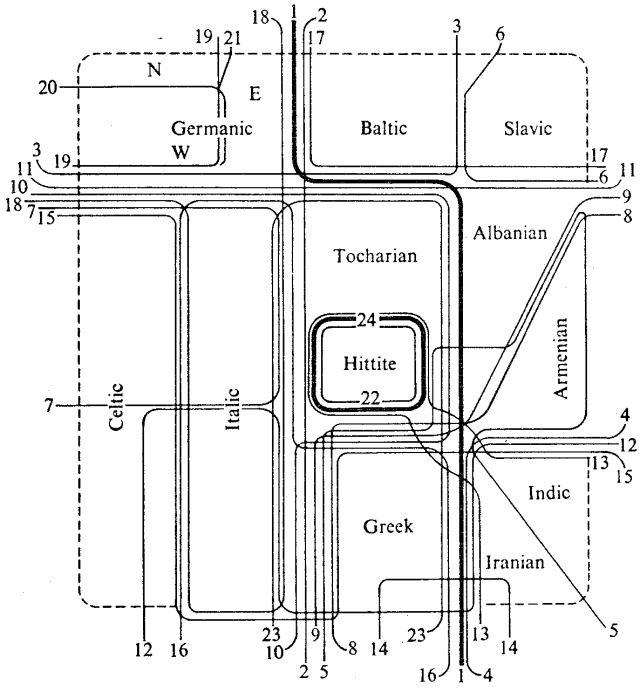
\includegraphics[scale=.6]{Indo.jpg}
\caption{The Wave Model of Indo-European Languages}
\label{fig:download}
\end{figure}

Given documentation of surviving cognates and similar forms, a computer can objectively create a tree model from the various linguistic data. 

\begin{figure}[h!]
\centering
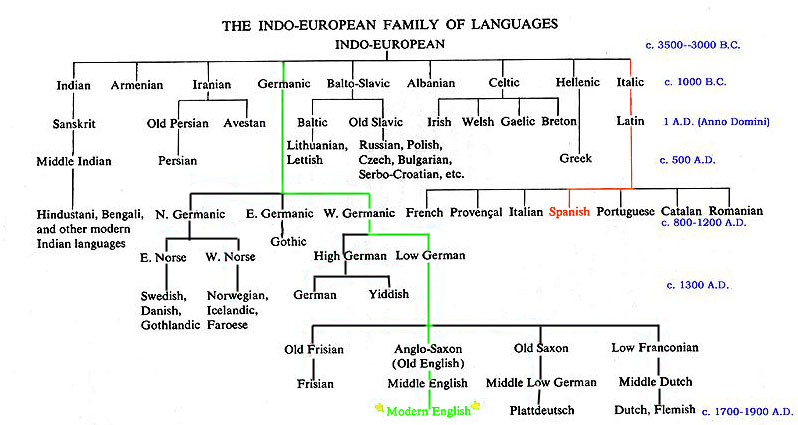
\includegraphics[scale=.6]{treemodel.jpg}
\caption{The Tree Model of Indo-European Languages}
\label{fig:download}
\end{figure}

\paragraph{Dialectology} Usually studied with maps that divide distributions with complimentary features. Compare geographical regions and linguistic trends. Examined by Neo-Grammarian to prove language change, ended up somewhat disproving it. 

``Rhenish Fan": an isogloss bundle that goes across northern Germany. (Rhine river between Germany and France). Fans out to a number of different isoglosses for different words. What was a regular change in Germany was irregular in the surrounding rural areas: some forms were shifted and others were not (unsystematic). 

\section*{Tuesday, 25 October 2016: Dialectology, Sociology}

\paragraph{Rhenish Fan (con't)}: Dialectology in models of linguistic change; wave vs. tree models. In lexical forms, you wouldn't necessarily expect isoglosses to all occur in the same place. When we see major glosses of all isoglosses, they indicate major dialectal divisions. Irregular change, steady along a river, ``fans out". Could be a result of many languages and contact in the region. River can be a barrier as well as an important channel of communication (only channel in pre-modern era). This is called a \textbf{transition zone}. Often the difference between two dialects is not clear-cut (except when communities are separated by a clear geographical barrier). This led for dialectologists to claim (contrary to Neo-Grammarian thought) that the unit of the change was the word, not the phoneme. 


\begin{figure} [h!]
    \centering
    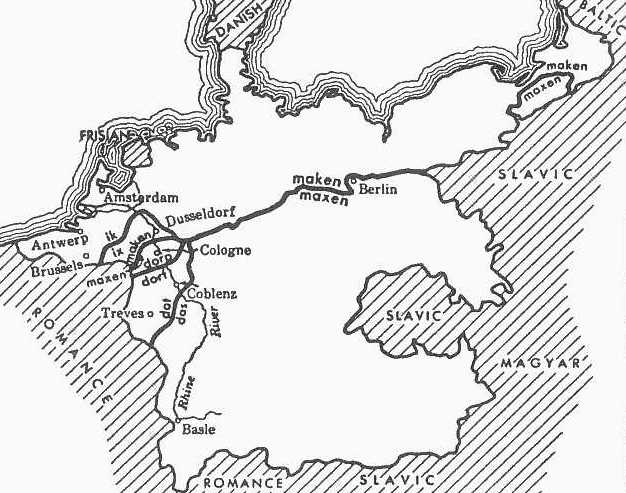
\includegraphics[scale=1.5]{rhenish_fan.jpg}
    \caption{Rhenish fan}
    \label{fig:my_label}
\end{figure}


\paragraph{Dialectology}Typically studied with dialect maps, which link dialects and their ling. features spoken to topographical features. Delimit isoglosses. Bundles of isoglosses with similar locations denote regional differences. 

A riff arose between Dialectology and Neo-Grammarians when Neo-Grammarians found that the regular sound change they expected to find were not so regular. Modern theoretical linguistics is the descendant of historical linguistics; preference for generalization and theoretical development. On the other hand, dialectology prefers empirical methods and focused on detail. 



Often, there was merit in both views. Changes were regular in some places, but changes were often unsystematic in the transition zone. (The Rhenish fan is an excellent example of this). 

Another example can be seen in the variety of r versus r-less varieties of English. Dialect maps allow us to track a change from its place of origin to its later diffusion. Instance of gradual diffusion on a generational basis. Some dialectologists don't beleive in dialects as an empirical reality. If we take the conclusion of all of these communities and transition zones. We only find `pure' dialects in an area well away from the transition zone, but in between those areas is a `mishmash', may better be represented as varying probabilities of different features rather than discrete dialects. We can only characterize communities as having the probability of using certain forms/structure. To assume that those frequencies can be extrapolated to a ``dialect" is an abstraction. To explain all irregularities and something that's NOT sound change is impossible. Both approaches have merit. Some changes are highly regular and some are not: both theories are relevant. 

\paragraph*{Sociolinguistics} Only very briefly discussed in textbook. To recap: until 1960s, most researchers thought it best to ignore synchronic variation, as it was assumed that it was only `white noise' that got in the way of making generalizations and theories. 

Chomsky: linguistics should be the study of the totally normal speaker in a homogeneous speech community. \textbf{Competence}, not \textbf{performance} should be studied. (\textit{Langue} more important than \textit{parole}, to use de Saussure's terminology). Many considered language change that was so slow and gradual as to be unobservable in real time. This was a major impediment to historical linguistics. 

The belief that variation was unprincipled (something to be sidestepped) was based on the assumption that the change was random and unpredictable. This view was challenged in the 1950s (John Fisher) and in the 1960s by William Labov (Martha's Vineyard and NYC department stores). Variation which appeared to be unsystematic was actually dependent on many social factors (like age, and social class); was actually an instance of \textbf{orderly homogeneity}. Predictable variations could account for the seemingly random variations between forms. (In NYC, high class people are less likely tto use formal -ing form, this probability becomes gradually less likely as style becomes more formal. Pronunciation also depends on the formality of a particular situation.) Entire community is involved in a common, but variable, element. 

This view of language was very different than Chomsky's view: it's clear that the  `ideal speaker in a homogeneous community' simply does not exist. Brings the need for lots and lots of data, as grammatical judgements cannot depend on one speaker's impression. 

\paragraph{Observer's Paradox} Best way to observe language is to observe it directly, yet observation causes the listener to speak in a different style (usually more formally) than they would have otherwise. The natural state of language occurs outside the laboratory. This can be merited by either collecting data in such a way that people aren't aware they're being studied. Or, you can distract people from their speech by asking to talk about something that's more emotionally engaging (for instance, by asking them to talk about a scary, funny, or happy memory). 

Labov found a significant difference between young and old speech styles. He extrapolated that synchronic variation was often the manifestation of diachronic change. As a change is occurring, you will have a time period in which some use the old form and some use the new form. The belief that language change was unobservable stemmed from the belief that synchronous variation was of no significance.

Labov: while not all variation indicates change, all change involves variation (for instance, some variation can remain stable for many generations without the overall population shifting from one form to another). 

Social diffusion similar to geographic distribution: spread from small group of innovators out to rest of community. Sometimes, these changes can cross language barriers as well as social ones.

\paragraph{Apparent Time Hypothesis} Merger: between aspirated and aspirated w phoneme (English). Distinction is gone in virtually all major and most dialects of English. Mapped, a higher and higher frequency uses identical forms. Our view of the 1920s depends on an assumption (the `apparent time' hypothesis: people maintain their grammar around the same time that they acquire it). Language acquisition shuts down at puberty, so grammatical patterns tend to remain fixed, suggesting that adult grammars are fixed (so, people in their 80s would reflect the language patterns they learned when they were around 10). By looking at a succession of these groups, we can get a picture of language change over time). 

\paragraph{Age Grading Hypothesis} However, this may not be the case: Age Grading Hypothesis suggests that people may switch their language with time. People may change their language over time as they enter different phases in life (for instance, a worker may adopt a new style of speaking to fit in in his workplace; a parent may swear less to make a good impression for his children; a parent may learn new change from his teenage son.

To reconcile the two: phonology and syntax may be more resistant to change than other areas, like morphology. For instance, adults can easily acquire new vocabulary when they learn about a new concept. 

S curve pattern is common in language change: they start of slowly over a long period of time, then pick up very quickly before leveling off again near the top. 

\begin{figure} [h!]
    \centering
    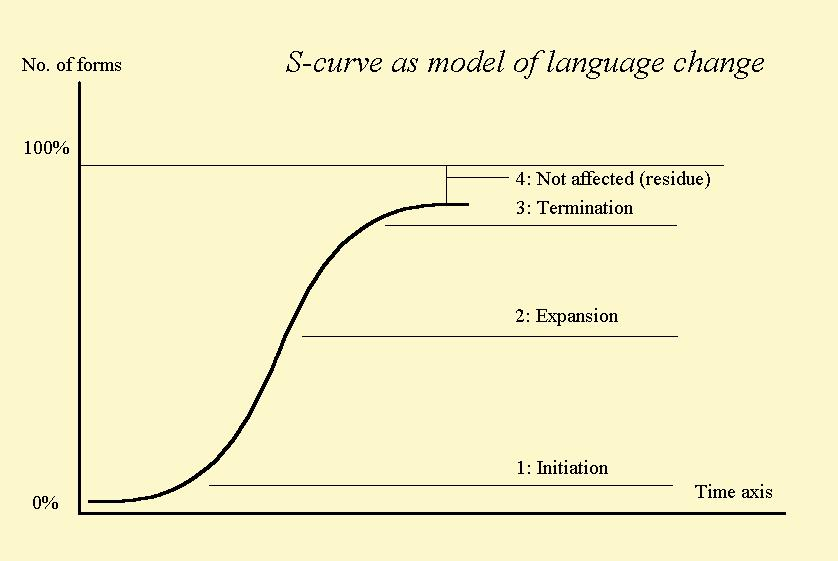
\includegraphics[scale=.4]{s_curve.JPG}
    \caption{S-Curve common of language change}
    \label{fig:my_label}
\end{figure}

\end{document}
